\documentclass[12pt, a4paper, fleqn]{memoir}%makeidx
\usepackage{lmodern}
\usepackage{chngcntr}

%******************************************************************************
% STYLE
%******************************************************************************
%******************************************************************************
% PACKAGES
%******************************************************************************
\usepackage{graphicx}
\usepackage{epsfig}
\usepackage{amsmath}
\usepackage{amssymb}
\usepackage{amsthm}
\usepackage{booktabs}
\usepackage{stmaryrd}
\usepackage{url}
\usepackage[figuresright]{rotating}
\usepackage{listings}
\usepackage{algorithm}
\usepackage{algpseudocode}
\usepackage{pifont}
\usepackage{ifsym}
\usepackage{relsize}
\usepackage[ansinew]{inputenc}
%\usepackage{dingbat}
\usepackage{hhline}
\usepackage{booktabs}
%\usepackage{xtab}
%\usepackage[margin=10pt,font={small,sf},labelfont=bf]{caption}
%\usepackage{tabularx}
%\usepackage{longtable}
%\usepackage{multirow}
\usepackage{color}
\usepackage{colortbl}
\usepackage{fancyvrb}
\usepackage{rotating}
\usepackage{makeidx}
\usepackage{MnSymbol}
\usepackage{textcomp}
%******************************************************************************
% INDEX GENERATION
%******************************************************************************
\makeindex

%******************************************************************************
% HYPEREF/ALGORITHM FIX
%******************************************************************************
\newcommand{\theHalgorithm}{\arabic{algorithm}}

% Konfiguration von hyperref
%\hypersetup{pdftex=true, colorlinks=true, breaklinks=true,
%   linkcolor=schwarz, menucolor=schwarz, pagecolor=schwarz, urlcolor=schwarz, citecolor=schwarz}

%******************************************************************************
% NUMBERING
%******************************************************************************
\numberwithin{algorithm}{chapter}
\numberwithin{figure}{chapter}

%******************************************************************************
% PAGE NUMBER IN BIBLIOGRAPHY
%******************************************************************************
\usepackage{citeref}
\renewcommand{\bibitempages}[1]{\newblock {\scriptsize [\mbox{cited at p.\ }#1]}}

%******************************************************************************
% PDF HYPERLINKS
%******************************************************************************
\ifpdf
  \pdfcompresslevel=9
        \usepackage[plainpages=false,pdfpagelabels,bookmarksnumbered,%
        colorlinks=true,%
        linkcolor=blue,%
        citecolor=blue,%
        filecolor=blue,%
        pagecolor=blue,%
        urlcolor=blue,%
        pdftex,
        unicode]{hyperref} 
    \input supp-mis.tex
    \input supp-pdf.tex
    \pdfimageresolution=600
    \usepackage{thumbpdf} 
\else
    \usepackage{hyperref}
\fi
\usepackage{memhfixc}

%******************************************************************************
% PAGE LAYOUT
%******************************************************************************
%\settypeblocksize{*}{32pc}{1.618}
%\setlrmargins{*}{1.47in}{*}
%\setulmargins{*}{*}{1.3}
%\setheadfoot{\onelineskip}{2\onelineskip}
%\setheaderspaces{*}{2\onelineskip}{*}
%\def\baselinestretch{1.1}
%\checkandfixthelayout



\newcolumntype{H}[1]{>{\columncolor[gray]{0.90}}p{#1}}
\newcolumntype{I}[1]{>{\centering\columncolor[gray]{0.90}}p{#1}}
\newcolumntype{q}[1]{>{\centering}p{#1}}
\renewcommand{\arraystretch}{1.25}
%******************************************************************************
% CHAPTER AND SECTION STYLE
%******************************************************************************
\makechapterstyle{mychapterstyle}{%
    \renewcommand{\chapnamefont}{\LARGE\sffamily\bfseries}%
    \renewcommand{\chapnumfont}{\LARGE\sffamily\bfseries}%
    \renewcommand{\chaptitlefont}{\Huge\sffamily\bfseries}%
    \renewcommand{\printchaptertitle}[1]{%
        \chaptitlefont\hrule height 0.5pt \vspace{1em}%
        {##1}\vspace{1em}\hrule height 0.5pt%
        }%
    \renewcommand{\printchapternum}{%
        \chapnumfont\thechapter%
        }%
}
\chapterstyle{mychapterstyle}
\setsecheadstyle{\Large\sffamily\bfseries}
\setsubsecheadstyle{\large\sffamily\bfseries}
\setsubsubsecheadstyle{\normalfont\sffamily\bfseries}
\setparaheadstyle{\normalfont\sffamily}
\makeevenhead{headings}{\thepage}{}{\small\slshape\leftmark}
\makeoddhead{headings}{\small\slshape\rightmark}{}{\thepage}

%******************************************************************************
% TABLE OF CONTENTS STYLE
%******************************************************************************
\settocdepth{subsection}
\setsecnumdepth{subsection}
\maxsecnumdepth{subsection}
\settocdepth{subsection}
\maxtocdepth{subsection}

%******************************************************************************
% COMMANDS FOR EPIGRAPHS
%******************************************************************************
\setlength{\epigraphwidth}{0.57\textwidth}
\setlength{\epigraphrule}{0pt}
\setlength{\beforeepigraphskip}{1\baselineskip}
\setlength{\afterepigraphskip}{2\baselineskip}
\newcommand{\epitext}{\sffamily\itshape}
\newcommand{\epiauthor}{\sffamily\scshape ---~}
\newcommand{\epititle}{\sffamily\itshape}
\newcommand{\epidate}{\sffamily\scshape}
\newcommand{\episkip}{\medskip}
\newcommand{\myepigraph}[4]{%
	\epigraph{\epitext #1\episkip}{\epiauthor #2\\\epititle #3 \epidate(#4)}\noindent}


%******************************************************************************
% FOOTNOTE STYLE
%******************************************************************************
\renewcommand{\thefootnote}{\fnsymbol{footnote}}

%******************************************************************************
% COLORS
%******************************************************************************
\usepackage{color}
\definecolor{greenyellow}   {cmyk}{0.15, 0   , 0.69, 0   }
\definecolor{yellow}        {cmyk}{0   , 0   , 1   , 0   }
\definecolor{goldenrod}     {cmyk}{0   , 0.10, 0.84, 0   }
\definecolor{dandelion}     {cmyk}{0   , 0.29, 0.84, 0   }
\definecolor{apricot}       {cmyk}{0   , 0.32, 0.52, 0   }
\definecolor{peach}         {cmyk}{0   , 0.50, 0.70, 0   }
\definecolor{melon}         {cmyk}{0   , 0.46, 0.50, 0   }
\definecolor{yelloworange}  {cmyk}{0   , 0.42, 1   , 0   }
\definecolor{orange}        {cmyk}{0   , 0.61, 0.87, 0   }
\definecolor{burntorange}   {cmyk}{0   , 0.51, 1   , 0   }
\definecolor{bittersweet}   {cmyk}{0   , 0.75, 1   , 0.24}
\definecolor{redorange}     {cmyk}{0   , 0.77, 0.87, 0   }
\definecolor{mahogany}      {cmyk}{0   , 0.85, 0.87, 0.35}
\definecolor{maroon}        {cmyk}{0   , 0.87, 0.68, 0.32}
\definecolor{brickred}      {cmyk}{0   , 0.89, 0.94, 0.28}
\definecolor{red}           {cmyk}{0   , 1   , 1   , 0   }
\definecolor{orangered}     {cmyk}{0   , 1   , 0.50, 0   }
\definecolor{rubinered}     {cmyk}{0   , 1   , 0.13, 0   }
\definecolor{wildstrawberry}{cmyk}{0   , 0.96, 0.39, 0   }
\definecolor{salmon}        {cmyk}{0   , 0.53, 0.38, 0   }
\definecolor{carnationpink} {cmyk}{0   , 0.63, 0   , 0   }
\definecolor{magenta}       {cmyk}{0   , 1   , 0   , 0   }
\definecolor{violetred}     {cmyk}{0   , 0.81, 0   , 0   }
\definecolor{rhodamine}     {cmyk}{0   , 0.82, 0   , 0   }
\definecolor{mulberry}      {cmyk}{0.34, 0.90, 0   , 0.02}
\definecolor{redviolet}     {cmyk}{0.07, 0.90, 0   , 0.34}
\definecolor{fuchsia}       {cmyk}{0.47, 0.91, 0   , 0.08}
\definecolor{lavender}      {cmyk}{0   , 0.48, 0   , 0   }
\definecolor{thistle}       {cmyk}{0.12, 0.59, 0   , 0   }
\definecolor{orchid}        {cmyk}{0.32, 0.64, 0   , 0   }
\definecolor{darkorchid}    {cmyk}{0.40, 0.80, 0.20, 0   }
\definecolor{purple}        {cmyk}{0.45, 0.86, 0   , 0   }
\definecolor{plum}          {cmyk}{0.50, 1   , 0   , 0   }
\definecolor{violet}        {cmyk}{0.79, 0.88, 0   , 0   }
\definecolor{royalpurple}   {cmyk}{0.75, 0.90, 0   , 0   }
\definecolor{blueviolet}    {cmyk}{0.86, 0.91, 0   , 0.04}
\definecolor{periwinkle}    {cmyk}{0.57, 0.55, 0   , 0   }
\definecolor{cadetblue}     {cmyk}{0.62, 0.57, 0.23, 0   }
\definecolor{cornflowerblue}{cmyk}{0.65, 0.13, 0   , 0   }
\definecolor{midnightblue}  {cmyk}{0.98, 0.13, 0   , 0.43}
\definecolor{navyblue}      {cmyk}{0.94, 0.54, 0   , 0   }
\definecolor{royalblue}     {cmyk}{1   , 0.50, 0   , 0   }
\definecolor{blue}          {cmyk}{1   , 1   , 0   , 0   }
\definecolor{cerulean}      {cmyk}{0.94, 0.11, 0   , 0   }
\definecolor{cyan}          {cmyk}{1   , 0   , 0   , 0   }
\definecolor{processblue}   {cmyk}{0.96, 0   , 0   , 0   }
\definecolor{skyblue}       {cmyk}{0.62, 0   , 0.12, 0   }
\definecolor{turquoise}     {cmyk}{0.85, 0   , 0.20, 0   }
\definecolor{tealblue}      {cmyk}{0.86, 0   , 0.34, 0.02}
\definecolor{aquamarine}    {cmyk}{0.82, 0   , 0.30, 0   }
\definecolor{bluegreen}     {cmyk}{0.85, 0   , 0.33, 0   }
\definecolor{emerald}       {cmyk}{1   , 0   , 0.50, 0   }
\definecolor{junglegreen}   {cmyk}{0.99, 0   , 0.52, 0   }
\definecolor{seagreen}      {cmyk}{0.69, 0   , 0.50, 0   }
\definecolor{green}         {cmyk}{1   , 0   , 1   , 0   }
\definecolor{forestgreen}   {cmyk}{0.91, 0   , 0.88, 0.12}
\definecolor{pinegreen}     {cmyk}{0.92, 0   , 0.59, 0.25}
\definecolor{limegreen}     {cmyk}{0.50, 0   , 1   , 0   }
\definecolor{yellowgreen}   {cmyk}{0.44, 0   , 0.74, 0   }
\definecolor{springgreen}   {cmyk}{0.26, 0   , 0.76, 0   }
\definecolor{olivegreen}    {cmyk}{0.64, 0   , 0.95, 0.40}
\definecolor{rawsienna}     {cmyk}{0   , 0.72, 1   , 0.45}
\definecolor{sepia}         {cmyk}{0   , 0.83, 1   , 0.70}
\definecolor{brown}         {cmyk}{0   , 0.81, 1   , 0.60}
\definecolor{tan}           {cmyk}{0.14, 0.42, 0.56, 0   }
\definecolor{gray}          {cmyk}{0   , 0   , 0   , 0.50}
\definecolor{black}         {cmyk}{0   , 0   , 0   , 1   }
\definecolor{white}         {cmyk}{0   , 0   , 0   , 0   } 
\definecolor{cell}          {cmyk}{0   , 0   , 0   , 0.25} 
\definecolor{stahlblau}		  {rgb} {0.2,0.56,0.84}
\definecolor{graurot}       {rgb} {0.62,0.15,0.15}
\definecolor{schwarz}       {rgb} {0.0,0.0,0.0}

\counterwithout{table}{chapter}

%******************************************************************************
% BEGIN DOCUMENT
%******************************************************************************
\begin{document}

%******************************************************************************
% FRONT MATTER
%******************************************************************************
\frontmatter

%******************************************************************************
% EMPTY PAGE
%******************************************************************************
\pagestyle{empty}
This is actually the first page of the thesis and will be discarded after the print out. This is done because 
the title page has to be an even page. The memoir style package used by this template makes different indentations 
for odd and even pages which is usually done for better readability. \cite{wagner2005physiological} 
\clearpage
%******************************************************************************
% TITLE PAGE
%******************************************************************************
\pagestyle{empty}
\rmfamily
\noindent
\begin{center}
University of Augsburg\\
Faculty of Applied Computer Science\\
Department of Computer Science\\
Master's Program in Computer Science\\
\end{center}
\begin{figure}[h]
\centering

\includegraphics[width=0.25\textwidth]{logo.png}
\end{figure}
\vfill\vfill
\begin{center}
\Large
Bachelor's Thesis\\
\end{center}
\vspace{2.0em}
\begin{center}
\Large
\LARGE Emotion Recognition\\ \vspace{10pt} 
\Large Supervised Classification of EEG Signals
\end{center}
\vspace{2.0em}
\begin{center}
    \normalsize
    submitted by\\
    \large
    Samy Shihata\\
    \normalsize
    on 28.6.2013
\end{center}
\vspace{2.0em}
\begin{center}
    \normalsize
    Supervisor:\\ 
    Prof. Dr. Elisabeth Andr\'{e} aus Augsburg
\end{center}
\begin{center}
    \normalsize
    Adviser:\\
    M.Sc. Johannes Wagner,
    M.Sc. Florian Lingenfelser 
\end{center}
\begin{center}
    \normalsize
    Reviewers:\\
    Prof. Dr. Elisabeth Andr\'{e}\\
\end{center}
\cleardoublepage

%******************************************************************************
% DEDICATION
%******************************************************************************
\vspace*{\fill}
{\hfill\sffamily\itshape} Dedicated to my family for their love and support. 
\cleardoublepage

%******************************************************************************
% ABSTRACT
%******************************************************************************
\chapter*{Abstract}
This thesis aims at investigating the use of EEG signals in classifying a user's emotional state, to prepare for integration into the Augsburg Biosignal Toolbox (AuBT\footnote{A Matlab toolbox for physiological signal analysis. More details at http://www.informatik.uni-augsburg.de/lehrstuehle/hcm/projects/tools/aubt/}). The data corpus is taken from the DEAP (Database for Emotional Analysis using Physiological signals) and used to solve three binary classification problems relating to affective state recognition. First, different approaches for feature extraction and selection are researched. Among those, the method of calculating the PSD (Power Spectrum Density), based on the FFT,  is selected due to its popularity and simplicity of implementation. For classification, three standard classifier are tested for cross comparing accuracy as well as comparison with results reported in previous works. The tests consists of two experiments, the first experiment uses the data for each subject separately for classification, before calculating the average classification accuracy over all subjects. This shows the expected rate of correct classification for a single user. The second experiment includes the entire data of all subjects as a single corpus for classification. This is done to demonstrate the generalizability of an EEG classifier for many users with different EEG patterns. Finally, a new classifier, previously proposed in the literature to be used in EEG classification, is implemented and tested. The thesis concludes with a comparison between the accuracies of tested approaches and future recommendations for further improvements. 

%******************************************************************************
% ACKNOWLEDGMENTS
%******************************************************************************

\chapter*{Acknowledgments}
I would like to express sincere gratitude to Prof. Dr. Elisabeth Andr\'{e} for offering this opportunity. Also, many thanks to my advisors Johannes Wagner and Florian Lingenfelser for their help and guidance, without which, this work would not have been done.
%Acknowledgements writing allows an author to tell some words of gratitude to those, who turned out to be rather helpful during your thesis writing process. Of course, acknowledgements are not an integral part of a thesis and if you did all your work on your own, you can omit this part. Writing acknowledgements is not obligatory.

%******************************************************************************
% STATEMENT & DECLARATION
%******************************************************************************
\chapter*{Statement and Declaration of Consent}
\vfill
\subsubsection*{\LARGE Statement}
Hereby I confirm that this thesis is my own work and that I have documented all sources used.
\vfill
\begin{flushleft}
Samy Shihata
\end{flushleft}  
\begin{flushright}
Augsburg, 28.06.2014 
\end{flushright}
\vfill
\vfill
\subsubsection*{\LARGE Declaration of Consent}
Herewith I agree that my thesis will be made available through the library of the Computer Science Department.
\vfill
\begin{flushleft}
Samy Shihata
\end{flushleft}  
\begin{flushright}
Augsburg, 28.06.2014 
\end{flushright}
\vfill

%******************************************************************************
% TABLE OF CONTENTS
%******************************************************************************
\cleardoublepage
\rmfamily
\normalfont
\pagenumbering{roman}
\pagestyle{headings}
\tableofcontents


%******************************************************************************
% MAIN MATTER
%******************************************************************************
\mainmatter

%##########################################################
\chapter{Introduction}
\label{chap:Introduction}

\section{Background}
\subsection{Affective Computing}
Affective computing is one of the rapidly growing fields of research in the disciplines of computer science, cognitive psychology and physiology \cite{tao2005affective}. It aims at expanding computers with the human like ability of dealing with emotions. This involves a two sided effort, for one a computer needs to be able to gather information about the user's emotional state. This needs to be done implicitly, without the user specifying his current state. A computer must learn to process such information and adapt appropriately to different emotions expressed by its users. On the other side, affective computing can also imbue computers, and machines in general, with ability to portray or simulate emotions and emotional responses \cite{picard2003affective, picard1999affective}. 

While not all machines would benefit from such capabilities, many situations can be improved by making the machine simulate a human agent's ability to naturally adapt to a given context \cite{picard1999affective}. At the spear head of such applications is human-computer interaction, which can be made much easier and more natural by introducing a  channel of emotional information between the user and the machine. This is analogous to the large amount of information passed to and from a person in human-human interaction, simply through voice tones, facial expressions and body language \cite{cowie2001emotion}. For example, a computer able to detect a user's frustration towards a certain GUI feature, can perhaps modify itself to be more suitable to the user's need, or simply offer a human like response to alleviate the user's frustration. Other application that would benefit from affective computing include data gathering for psychological research, such as collecting data on frustration expressions, development of tools for training of social-emotional skills and building service robots able to interact with people in a nursing or shopkeeping capacity \cite{picard1999affective}.

\subsection{Electroencephalography}
Modern medicine uses a variety of techniques to capture and record different activities of the human body. One of those techniques, known as Electroencephalography (EEG), has undergone massive progress in recent years. The current procedure of EEG entails the use of electrically conductive electrodes to detect electrical activity produced by the brain. When a large number of brain cells are activated, a local electric current starts flowing, which can cause faint electrical signals to manifest on the scalp. Once these signals are captured by the electrodes, they can be displayed on paper, or recorded to computer memory for further processing. Electroencephalographic reading can be done in two ways, called invasive and non-invasive procedures. The invasive form requires a surgical procedure to implant electrodes directly on the surface of the brain (subdural EEG) or within the substance of the brain (depth EEG). In the non-invasive EEG procedure, electrodes are placed over the subject's scalp without the need for surgery or incision. While the non-invasive procedure requires more sensitive sensors and is more prune to noise and interference, it is much more practical than the invasive counter part. It can be applied many times to both adults and children without any risk of injury or brain damage \cite{teplan2002fundamentals}. For the purpose of this study, the term EEG will always refer to signals recorded by a non invasive procedure.

EEG signal recording has its long established uses in the fields of neurology and clinical neurophysiology. This is due its ability to reflect both normal and abnormal brain activity. It can also record the brain response to a stimuli within fractions of a second of its occurrence. This allows for a long list of applications including monitoring brain alertness, coma, brain death and certain brain disorders such as epilepsy. However, recently, more focus has been given to the specific problem of computer classification of EEG signals using techniques such as machine learning. The main goal behind such research is the development of Brain Computer Interfaces (BCIs). These interfaces allow users to communicate simple commands to different machinery using nothing but brain signals. This can be invaluable to a disabled person with no motor skills (such as patients with spinal cord injury). EEG signal classification has also been used in the verification of theoretical hypotheses regarding the inner workings of the brain. Despite the major advances made in the field, there has been little attention given to the use of EEG signals in determining a subject's emotional state. This contribution aims at using new as well as previously developed techniques of EEG signal classification into affective state detection (recognition of human emotions). 
\section{Motivation}
\label{sec:Motivation}
This work is part of an ongoing effort to develop a Matlab toolbox, called the AuBT (Augsburg Biosignal Toolbox), for the recognition of human emotions through physiological signal analysis. Here, I attempt to expand on the existing components by adding an extra channel of sensors for capturing EEG signal and using the new input for interpreting the affective state of the subject. The toolbox, including this contribution, is expected to benefit many applications, such as the use of humanoid avatars where advanced human computer interaction is required. It can also be used for studies regarding human psychology and emotional behaviours.
\section{Objectives}
\label{sec:Objectives}
This study aims at investigating the use of EEG signals for determining the emotional state of a subject. It uses popular machine learning techniques as well as newly developed algorithms for the recognition of a subject's affective state. The data used for the study is the DEAP dataset, the first dataset to record the physiological state of several subjects as well as their self reported emotional response to certain music videos. 
\section{Outline}
\label{sec:Outline}
This study is divided into six chapters: introduction, dataset and preprocessing, feature extraction, classification, experimental results and a summary. This chapters are organised in the same order as what is normally the natural flow of machine learning problem. The fifth chapter, experimental results, reports the classification accuracies achieved in two experiments that were done during the course of the study and compares these results with previous experiments done with the same dataset. All implementations and experiments where done in Matlab using the AuBT$^{*}$ (Augsburg Biosignal Toolbox).

%##########################################################
\chapter{Electroencephalography}
\label{chap:Electroencephalography}

\section{History}
The discovery of electroencephalography was first made in 1875 by English physician, Richard Caton, who reported measuring what he described as ``feeble currents of varying directions'' from the exposed brains of rats and monkeys. The non-invasive procedure was then introduced by Hans Berger, a German neurologist, in 1924 who used ordinary radio equipment to amplify electrical activity produced by the brain on the human scalp. He used a strip of paper to show that EEG can be visually inspected without the need to open the skull.

\section{Technical Details}

\begin{figure}[h]
	\centering
	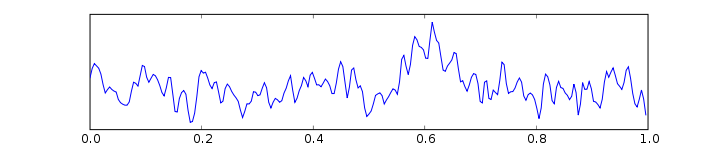
\includegraphics[width=0.8\textwidth]{eeg.png}
	\caption{Raw EEG signal, 1 second recording}
\end{figure}
Potential Difference is formed in brain neurons with the flow of Ca$^{++}$, K$^{+}$, Na$^{+}$ and Cl$^{-}$ -ions through membrane channels. The potential difference can either exceed a threshold making it an action potential or be subthreshold as post synaptic potentials (PSPs). Action potentials are spike shaped with duration of 1 ms that, when responding to stimuli that exceed a certain threshold, causes the neuron to fire. When action potentials reach a synapse, a connection between the firing neuron and other neurons, it forms a PSP with amplitude relative to the excitation of the input neuron. PSPs have typical amplitudes ranging from 5-10mV and spans between 10 and 50 ms. These potentials propagate throughout the brain neurons in same way. When that number of firing neurons causes a large enough PSP, extracranial electric field is formed. The contribution of action potentials to this field is negligible. The superimposition of post synaptic potentials detected is known as EEG.

EEG is recorded by means of conductive electrodes placed on the scalp. Conductive paste and low resistance electrode can be used to boost recording quality. The need to interpret single recordings as well as compare results call for standardized placement of electrodes. In 1958, a standard for electrode placement was introduced, called 10-20 electrode placement system. Using proportional distances from skull landmarks, the 10-20 system provides adequate coverage of the entire scalp. The name 10-20 stands for the percentages of distances between the ears and nose where electrode positions where chosen. Each electrode position is given a label based on the closest brain area: (F)rontal, (C)entral, (T)emporal, (P)osterior and (O)ccipital. On the left side of the brain, from the subjects perspective, labels are accompanied by an odd number on the left side and an even number on the right.

\section{Applications}
The dedicated research effort behind EEG measurement is motivated by the very wide spectrum of applications it offers. EEG holds an advantage over other brain monitoring techniques in its high speed. It allows the recording of a stimuli response within fractions of a second of its occurrence. Clinical applications include anaesthesia, testing for drug effects, examining the brain for tumors or strokes and monitoring patients with coma or brain death. Certain variation of EEG signals can be used for specific applications. For example, evoked potentials can be used for cognitive related studies. Quantitative electroencephalography, the use of multi channel measurements of EEG, is typically used for topographic brain mappings. A popular application which has gained attention recently is Brain Computer Interfaces (BCI). BCIs are computer interfaces designed to translate EEG signals from a user into simple commands from a preprogrammed set. This allows users with little or no mobility, such as patients with neck-down-paralysis, to control daily objects with nothing but brain commands.

\chapter{Data Used}
\label{chap:dataset}

\section{Dataset Source and Construction}
\label{sec:DatasetSource}
The continued research in the field of emotion recognition has called for the creation of many databases for physiological recordings. Existing databases cover many different modalities such as facial expressions, body gestures and speech. The dataset used for this study is a database called, DEAP (Database for Emotional Analysis using Physiological signals), that was first presented in 2012. It holds recordings of a large number of physiological signals, including EEG, and facial expressions of several subjects while using musical videos as emotional stimuli. The database also holds the subjects' self evaluation of their emotional state during each video with regards to: arousal, valence, dominance, liking and familiarity \cite{koelstra2012deap}.

Following is a summary of the procedure that went into the creation of the database\footnote{For more details the reader is referred to \cite{koelstra2012deap}}. It started with 120 musical videos, half of which were selected automatically and the rest manually. To ensure diversity, the manually selected videos were chosen such that each 15 videos belonged to a different quadrant in the valence/arousal space (LALV, LAHV, HAHV, HALV). Then for each video, a one minute highlight segment was extracted automatically through a linear regression method used in \cite{soleymani2009bayesian} to maximize the emotional content. An online subjective emotion assessment interface allowed users to evaluate the videos for arousal and valence. The final 40 videos were selected from the ones having the highest rating in terms of valence/arousal. These videos were viewed, in random order, by 32 subjects while their physiological state was recorded. For 22 subjects, facial expressions were also recorded. For each video, the subject provided a self assessment of their emotional state using self-assessment manikins (SAMs) in terms of valence, arousal, dominance and liking \cite{koelstra2012deap}.

\section{Recorded Signals and Preprocessing}
\label{sec:preprocessing}

\begin{figure}[h]
	\centering
	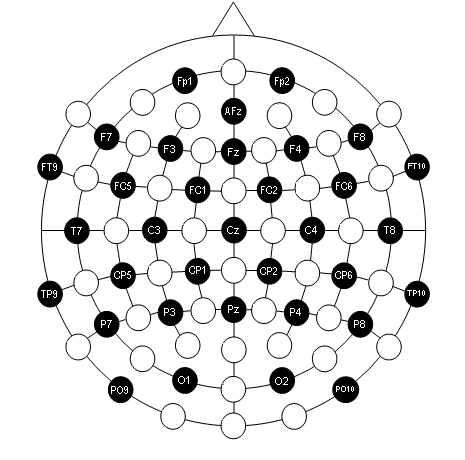
\includegraphics[width=0.6\textwidth]{pic.png}
	\caption{The 10/20 placement of electrodes from the DEAP dataset}
	\label{fig:eeg}
\end{figure}

The DEAP dataset was selected for its abundance in physiological information. The database holds recordings of 40 physiological signals, of which 32 are EEG channels. Figure \ref{fig:eeg} shows the 32 EEG channels and their positions on the scalp. The label of each channel and position are defined by the 10 - 20 system. While other physiological signals are included in the database, only EEG signals are considered in this study. Other than the large number of  data channels, the database's large number of subjects is another advantage. It has been noted that EEG signal patterns vary greatly among different individuals, and so the presence of data from that many subjects allow for testing emotional recognition techniques for generalizability.The database also provides preprocessed versions of the raw data to allow for a quick implement-and-test approach. Preprocessing used included down sampling from the original 512Hz to 128Hz, removal of EOG artefacts, bandpass frequency filtering between 4.0hz and 45.0hz and averaging the data to the common reference.

\chapter{Feature Extraction}
\label{chap:FeatureExtraction}

\section{Challenges and Typical Approaches}
\label{sec:CommonMethods}
Feature extraction is usually the first step in a classification problem. It is also the most crucial step as classification accuracy is naturally dependent on the quality of features used. This means that features need to be informative, discriminative between classes and descriptive of each class. The difficulty in feature extraction lies in the nature of an EEG signal which challenges most of the standard feature extraction techniques. The first complication that can be observed in EEG signals is the signal-to-noise ratio which tends to be very low. Second, EEGs are non stationary signals and experience sharp variations over time. This makes time related information, while essential to the recognition of stimuli related changes, very difficult to extract. Also, EEG classification lends itself easily to the curse of dimensionality and over fitting. This is caused by the large number of features extracted from multi channel sensor recordings. Adding to the problem, is the small size of the datasets usually available for training \cite{lotte2007review}.

Many techniques have been developed in order to improve the quality of extracted features. Commonly used, are the parametric methods such as the autoregressive(AR) and the adaptive autoregressive(AAR). These methods assume that the signal follows a mathematical model, whose exact form can be determined by estimating values for the free coefficients. The difference between the adaptive and the non-adaptive method is that an adaptive model is updated for each new sample arrival \cite{pardey1996review}. Other features include time frequency features, inverse model features, power spectrum density (PSD), and Band Powers(BP).

\section{Power Spectral Density}
\label{sec:psd}
The Power Spectrum Density (PSD) approach has been shown to outperform most other feature extraction techniques \cite{du2004temporal}. That and the simplicity of implementation are the reasons for choosing it as the feature extraction method. The process of calculating the power spectrum density is known as spectral power estimation. It means determining the power of the signal at each of several frequency bands. This splits the raw EEG signal into several much more informative values. Spectral estimation can be done in several ways. The simplest method is to apply a bandpass filter with the required bandwidth to the signal. The calculated power of the output signal divided by the bandwidth of the filter is the spectral density for that particular band. While straight forward, this approach is impractical for situations with a large number of frequency bands due to its slow performance. Other approaches to spectral density estimation are split into two groups, parametric and non-parametric methods \cite{stoica2005spectral}.

The parametric approach requires a model be fitted to the data. This means that the parametric approach requires the assumption that the signal is produced by a linear system driven by white noise. In the cases where the data truly follows the fitted model, the parametric approach can provide more accurate results. In other cases, however, this approach is quite sensitive to misspecification. In the non-parametric approach, the PSD is estimated directly from the signal. The most basic of the non-parametric methods is the Periodogram. This method uses the discrete-time Fourier transform of the signal, using the Fast Fourier Transform (FFT). The PSD in this case is the appropriately scaled magnitude squared of the result.
For a signal of L samples, the Periodogram is
$$P_{xx}=\frac{1}{LF_s}|\sum_{n=0}^{L-1}x_L^{(n)e^{\frac{-j2\pi fn}{F_s}}}|^{2}$$
Where $F_s$ is the sampling frequency.
The method used here is a variation of the Periodogram, known as the Welch Periodogram. Instead of calculating a Periodogram for the whole signal, the signal is first divided into segments of fixed size, that may overlap, and then a Periodogram is calculated for each segment separately. The results are then averaged to calculate the final PSD. This reduces variation and provides a smoother Periodogram \cite{john1996digital}.

\section{Extracted Features}
\label{sec:ExtractedFeatures}
Spectral density estimation was applied to each channel of EEG separately. Six frequency bands were considered, all belonging to the standard EEG nomenclature. Each of these bands have been shown to have strong correlation with a specific change in the mental state of the subject. They are the following:\\
\\
\textbf{Delta Waves} Frequency range lies between 0.1 and 4 Hz. They are clearly observed during episodes of deep sleep, known as slow-wave sleep, with large amplitudes, commonly between 75 and 200 $\mu V$.\\
\\
\textbf{Theta Waves} These are more commonly observed in children, and are rare in case of adults. They have been tied to states of light sleep or meditation. Their frequency range is between 4 and 8 Hz.\\
\\
\textbf{Alpha Waves} These waves mostly originate in the posterior part of the brain. They are observed during states of relaxed meditation. They become more prominent when the eyes are closed. It was observed that alpha waves are slightly blocked by mental effort or spiked attention. Frequency range lies between 8 and 12 Hz.\\
\\
\textbf{Slow Alpha Waves} Also known as the alpha delta waves, they are a special type of alpha waves. Their frequency range is restricted between 8 and 10 Hz and are dominant in the anterior-posterior gradient.\\
\\
\textbf{Beta Waves} Beta frequency range is much wider than other waves, between 12 and 30 Hz. Their spikes are related to increased attention, alertness and focus. Beta waves are suppressed right before and during physical motions.\\
\\
\textbf{Gamma Waves} Frequency range is above 30 Hz but rarely exceeds 45 Hz. Gamma waves are associated with higher mental functions, specifically the processing of information and voluntary movements.\\
\\
The power values of these six frequency bands were calculated for each of the 32 recorded channel and then concatenated into a single feature vector. This gives a feature vector of 192 features.

\begin{figure}[p]
	\centering
	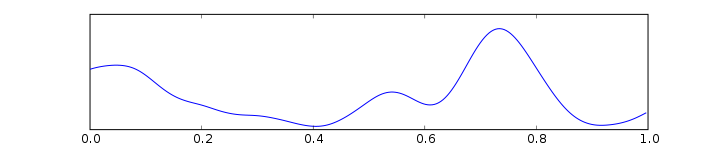
\includegraphics[width=0.8\textwidth]{eeg_delta.png}
	\caption{Delta wave, 1 second recording.}	
\end{figure}

\begin{figure}[p]
	\centering
	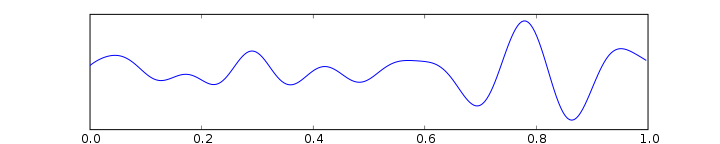
\includegraphics[width=0.8\textwidth]{eeg_theta.png}
	\caption{Theta wave, 1 second recording.}	
\end{figure}

\begin{figure}[p]
	\centering
	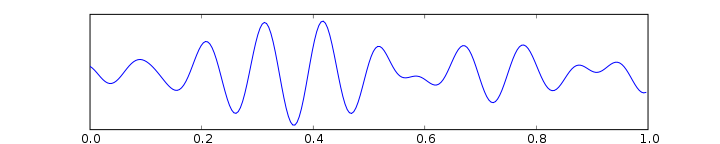
\includegraphics[width=0.8\textwidth]{eeg_alpha.png}
	\caption{Alpha wave, 1 second recording.}	
\end{figure}

\begin{figure}[p]
	\centering
	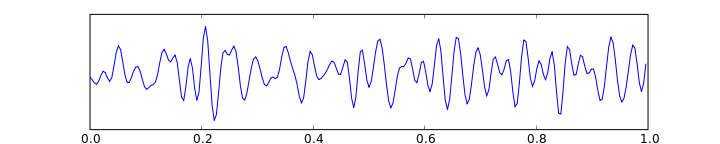
\includegraphics[width=0.8\textwidth]{eeg_beta.png}
	\caption{Beta wave, 1 second recording.}	
\end{figure}

\begin{figure}[p]
	\centering
	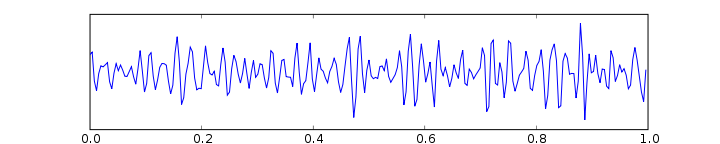
\includegraphics[width=0.8\textwidth]{eeg_gamma.png}
	\caption{Gamma wave, 1 second recording.}	
\end{figure}

\newpage
Other than the power spectral density, values spectral asymmetry were also used as features. Spectral power asymmetry is defined as the difference in power between the channels on the left and right hemispheres of the brain. That is to say that for each sensor channel on the right brain hemisphere, the corresponding symmetrical channel on the left hemisphere is identified. Then the power of the signals coming from both sensors is subtracted from each other. This is calculated for each of the above mentioned frequency bands. Spectral asymmetry values has been shown to be effective features in the recognition of certain mental disorders and tumors. With 14 symmetrical channels present in the data, the number of added features is 84 which extends the feature vector to 276 total features.

\section{Feature Selection}
\label{sec:FeatureSelection}
Following feature extraction, feature selection is applied. Feature selection is the process of selecting a subset of the available features to be actually used in classification. There are several benefits to feature selection. First, it can eliminate noisy features which merely confuse the classifier. It can improve the efficiency of classification by reducing storage space and training time.It can also remove features that are non discriminative between classes making them ineffectual to classification. Feature selection can greatly reduce the effect of the curse of dimensionality. This can be very important in EEG classification due to the normally small datasets. Many algorithms exist for feature selection. The method used here is called the Analysis of Variance (ANOVA). This is a statistical method commonly used to investigate the relations between samples. Here, it shows the contribution of each feature to the overall variance of the data. This restricts the feature set to the highest contributing features. This study compares between the accuracies of different classifiers with and without the use of feature selection \cite{guyon2003introduction}.

\chapter{Classification} 
\label{chap:Classification}

\section{Standard Classifiers}
\label{sec:StandardClassifiers}
For classification of the selected features, three standard classifiers were used: linear discriminant analysis (LDA), $k$ nearest neighbours (KNN) and multi-layered Perceptron. These classifiers have been used in many works relating to EEG classification and are described below:\\
\\
\textbf{LDA} The LDA is a statistical method that was introduced by RA Fisher \cite{fisher1936use}. When applied to a binary classification problem (containing two classes), the means of both classes, $\mu_1$ and $\mu_2$, and the covariances, $\sum_1$ and $\sum_2$, are calculated from the training set. The mean and covariance of each class serves as a representation of that class. The LDA makes the assumptions that both classes are normally distributed, and that both variances are equal ($\sum_1 = \sum_2 = \sum$). With that the decision function for class 1 becomes 
$$\vec{w} \cdot \vec{x} > T $$
Where $\vec{x}$ is a feature vector, $T$ is a constant threshold and 
$$\vec{w} \propto \sum\nolimits^{-1}(\mu_1 - \mu_2)$$
LDA can be applied to classification problems with more than 2 classes using the 1-vs.-all method \cite{hunterberger2003brain}.\\
\\
\textbf{KNN} This algorithm uses a form of majority vote to form a decision. To classify a feature vector $\vec{x}$, a set of the $K$ closest vectors is created and $\vec{x}$ is assigned to the most occurring class in the set. The determination of the closest vectors can be done using several distance metrics. The most commonly used distance measure is the Mahalanobis distance which, for two vectors $\vec{x}$ and $\vec{y}$, is equal to
$$d^2 = (\vec{x} - \vec{y})\sum\nolimits^{-1}(\vec{x} - \vec{y})^{T}$$
Where $\sum$ is the covariance matrix. KNN has the advantage of non linear decision boundary as it can approximate any function, providing $K$ is large enough. It benefits the most from feature selection as it is highly susceptible to the curse of dimensionality \cite{lotte2007review}.\\
\\
\textbf{MLP} This is a form of neural networks that simulates brain neurons. An MLP is formed of several connected nodes, where each connection has a weight. The input nodes receive the values of the feature vector, normalize them between 0 and 1 and then passes them to the next connected nodes. The values are multiplied by the connection weight before the process is repeated at the next node. Information propagate through the network using the same way until it reaches the output nodes. The output nodes produce the final values that determine the decision of the network. Neural network are known as universal approximators for their ability to approximate any function. This makes them somewhat sensitive to noise. Despite that, neural networks have been shown to be a very efficient classification technique and have been used in many BCI implementations.\\
\\

\section{Gaussian Classifier}
\label{sec:GaussianClassifier}

\subsection{Classifier Implementation}
The Gaussian classifier is the fourth classifier implemented to compare its performance with the other standard classifiers in EEG recognition. This classifier was developed specifically for use in brain computer interfaces for EEG classification. It was introduced in the work of Mill\'{a}n et al. (2000) \cite{millan2000local}. It was termed a ``a local neural classifier''. While its correct recognition rate can be outdone by other more standard classifiers, it holds two advantages that makes it more appropriate to online classification. First, it has very small resolution time (half a second) which can be essential for the classification of a continuous data streams. Second, the classifier has a lower wrong response rate than most other classifiers which can be important if the cost of recovery from a wrong classification is much higher than the cost of rejecting an uncertain sample. It is worth mentioning that this advantage is more relevant to applications of EEG based control than in EEG based emotion recognition.

For $N_k$ class classification problem, the algorithm for the Gaussian classifier starts by calculating the initial mean $\mu_k$ and covariance matrix $\sum_k$ of each class $C_k$ using the maximum likelihood approach
\begin{equation} \label{eq:mean}
	\mu_k = \frac{1}{N_k}\sum_{n=1}^{N_k}x^n
\end{equation}
\begin{equation} \label{eq:cov}
	\sum_k = \frac{1}{N_k}\sum_{n=1}^{N_k}(x^n - \mu_k)(x^n - \mu_k)^T
\end{equation}
With the assumption that each class has an independent normal distribution and using the values calculated above, the discriminant function for the classifier becomes
\begin{equation} \label{eq:yk}
	y_k(x) = \frac{-1}{2}(x - \mu_k)^T\sum\nolimits_k^{-1}(x-\mu_k)-\frac{1}{2}ln|\sum\nolimits_k|+lnP(C_k)
\end{equation}
Where $P(C_k)$ is the prior probability of class $C_k$. Here, the classes are considered to have equal probability of $\frac{1}{N_k}$. The discriminant function follows from the Bayesian rule
$$y_k(x) = P(C_k|x) = \frac{p(x|C_k)P(C_k)}{p(x)}$$
after dropping constant terms.

Practically, what this means is that the mean $\mu_k$ and covariance $\sum_k$ form a prototype for class $C_k$. During classification the sample $x$ is assigned to the closest prototype which is determined based on the Mahalanobis distance. During training the values of $\mu_K$ and $\sum_k$ are optimized iteratively using gradient descent to minimize the mean square error function. With the additional assumption of diagonal covariance matrices, the update function of $\mu_k$ for each feature vector $x^n$ becomes
\begin{equation} \label{eq:deltamu}
	\Delta \mu_k = \alpha[t_k(x^n)-y_k(x^n)]\sum\nolimits_k^{-1}(x^n-\mu_k)y_k(x^n)y_j(x^n)
\end{equation}
Where $t_k$ is the $K^{th}$ component of the target vector of the form 1-of-c, $yk$ is the probability of class $C_k$ calculated using \ref{eq:yk} and $y_j$ the probability of other classes. The values of the covariance matrices are reevaluated using \ref{eq:cov} after every full iteration over the training set.

\subsection{Shrunken Covariance}
A complication that arises from the large dimensionality of the feature vector, is the accuracy of covariance matrix estimation. With the number of features much greater than the number of samples in the dataset, calculated covariance matrix tend to be singular. The problem with a singular covariance matrix is that the inverse $\sum\nolimits^{-1}$, which is required for the calculation of yk given by \ref{eq:yk}, non existent. The solution that was implemented is the shrunken covariance matrix. The concept of a shrunken covariance matrix reduces the estimation errors by pushing the matrix towards a more structured form, the target matrix, where the diagonal elements are the sample variances \cite{disatnik2007shrinking}. The advantage of the target matrix is that it is guaranteed to be non singular (invertible), however, it can be a much worse estimation for the covariance matrix than the maximum likelihood estimation. For covariance matrix $S$, the shrunk covariance matrix $\sum\nolimits_{shrunk}$ is
\begin{equation}
	\label{eq:shrunkcov}
	\sum\nolimits_{shrunk} = \delta F + (1 - \delta)S
\end{equation}
Where $F$ is the target matrix and $\delta$ is a number between 0 and 1 called the shrinkage factor. The shrinkage factor effectively determines the contributions of the maximum likelihood estimation matrix $S$ and the target matrix $F$ to the final covariance matrix $\sum\nolimits_{shrunk}$. The shrinkage factor here is empirically determined to be 0.2. The elements of the target matrix $F$ can be calculated by 
\begin{equation}
	\label{eq:f}
	f_{ii} = s_ii
\end{equation}
\begin{equation}
	f_{ij} = \bar{r}\sqrt{s_{ii}s_{jj}}
\end{equation}
and $\bar{r}$ is the sample correlation given by
\begin{equation}
	\label{rbar}
	\bar{r} = \frac{2}{(N - 1)N}\sum^{N-1}_{i=1}\sum^{N}_{j=i+1}\frac{s_{ij}}{\sqrt{s_{ii}s_{jj}}}
\end{equation}
N is the number of samples in the dataset \cite{ledoit2004honey}.

\chapter{Experimentation and Results}
\label{chap:results}

\section{Setup}
\label{sec:setup}
Throughout the course of this study, two classification experiments were carried out in order to compare the performances of different classifiers and procedures on EEG signals. The setup of the two expermints closely resembles that which is used in \cite{koelstra2012deap}. Specifically, the first experiment follows the exact same procedure, while using different classifiers, to allow comparison of the produced results with the results reported in their work. To prepare for the expermints the signals are split into one minute segments, representing the recording of an EEG signal from a single subject while watching one musical video. This gives 40 segments for each of the 32 subjects making a total of 1280 segments. Each segment is considered a single sample in the dataset. Classification of a sample in this context indicates the overall emotion of the subject during a single musical video. This is preferable to the more common practice of using one second segments, as it provides a more meaningful classification rather than just indicate fluctuations in the  emotional state. Both experiments include three binary classification problems: arousal, valence and liking. Each sample in the dataset is classified into the three categories as either high or low. Since the DEAP dataset provides numerical values between 0 and 9 for the three categories, values higher than 4.5 are considered high.

\section{Experiment One}
\label{sec:exp1}
The first experiment is a standard classification experiment. The EEG samples from each of the 32 subjects is treated as a single training corpus. The four classifiers are then applied to the corpus for each of the three classification problems. The resulting correct classification and percentage accuracy is recorded. This procedure is then repeated for the 32 subjects, and the average accuracy of the four classifiers over all subjects is calculated. The validation theme used is the leave-one-out method, where one sample of the dataset is used as the testing sample and the rest as the training set. Validation is repeated until all samples are used as a testing set once, and the average test result is reported. This showcases the expected performance of each classifier when integrated into real life applications. The procedure of this experiment matches the single trial classification experiment carried out in \cite{koelstra2012deap} using a Na\"{\i}ve Bayes classifier. This is why the results reported in their work was included in the comparison of the results reported here. Only results that made use of feature selection were reported in their study.

\begin{table}[!h]
	\begin{tabular}{| c | c | c | c | c | c |}
		\hline \hline
		Emotion					& LDA	  & KNN	    & MLP     & Gaussian & NB      \\
		\hline \hline
		Arousal (without feature selection)	& 55.59\% & 59.25\% & 59.61\% & 56.44\%  & n/a     \\ \hline
		Arousal (with feature selection)        & 50.61\% & 51.72\% & 54.44\% & 50.00\%  & 62.00\% \\ \hline
		\hline
		Valence (without feature selection)     & 55.15\% & 64.48\% & 60.75\% & 57.86\%  & n/a     \\ \hline
		Valence (with feature selection)	& 49.77\% & 57.25\% & 60.29\% & 50.00\%	 & 57.00\% \\ \hline
		\hline
		Liking  (without feature selection)	& 54.24\% & 56.85\% & 59.57\% & 57.27\%  & n/a     \\ \hline
		Liking  (with feature selection)	& 49.77\% & 57.25\% & 60.29\% & 50.00\%  & 55.40\% \\ \hline
		\hline
	\end{tabular}
	\caption{Averages of correct classification percentages for experiment one}
	\label{table:exp1}
\end{table}

Table \ref{table:exp1} shows the averages of performance of the four classifiers over the 32 subjects. The Na\"{\i}ve Bayes classifier results are taken directly from \cite{koelstra2012deap}. The percentages are the ratio of correct classifications to the total classifications attempted. The results allow for comparisons between performances. While it can not be claimed that one classifier is completely superior to the others, it can be seen that the MLP has a relatively consistent high performance which can be attributed to its highly flexible decision boundary. This gives MLP an advantage in noisy data such as the EEG signals. It is also worth noting that not all classifiers benefit from adding feature selection, and in some other cases the improvement is not worth the added time complexity. The severe drop in the performance of the Gaussian classifier when using feature selection is caused by the greatly reduced number of features. The estimation of prototypes for classes requires a minimum number of features depending on the number of available samples in the training set. A possible solution to this problem is to dynamically determine the optimal shrinkage factor using gradient descent. Regarding the overall performances of the four classifiers, it can be seen that the correct prediction rate is comparable to those that are reported from the Na\"{\i}ve Bayes classifier in \cite{koelstra2012deap} and in other similar works. Still much improvement is needed before these rates can be depended on in practical applications.

\section{Experiment Two}
\label{sec:exp2}
One of the recurring problems in EEG classification is the sharp variation between different samples, which can greatly reduce the generalizability of results. This is not only true for data from different subjects, but also applies for data from the same subject that was acquired in different recording sessions. This has made it a standard practice to use classifier systems that are optimized for specific individuals. This may have had its uses in an academic environment, despite the added cost to calibration times and reproducibility. However, all attempts of applying such techniques to practical commercial applications remain highly unlikely without the development of more general solutions. To that end, this experiment was designed to compare the robustness of different classifiers, and to test the generalizability of their accuracies. The experiment uses the data of all 32 subjects as a single training corpus, with no indication of the different sources. The four classifiers are applied to the corpus in the same way as the previous experiment, for the three emotions with and without using feature selection.

\begin{table}[h]
	\begin{tabular}{| c | c | c | c | c |}
		\hline \hline
		Emotion 				& LDA     & KNN     & MLP     & Gaussian \\
		\hline \hline
		Arousal (without feature selection)     & 48.55\% & 52.87\% & 54.45\% & 48.83\%  \\ \hline
		Arousal (with feature selection)	& 47.51\% & 46.25\% & 52.32\% & 45.41\%  \\ \hline
		\hline
		Valence (without feature selection)	& 51.31\% & 48.96\% & 51.67\% & 52.82\%  \\ \hline
		Valence (with feature selection)   	& 46.67\% & 45.06\% & 43.95\% & 49.24\%  \\ \hline
		\hline
		Liking  (without feature selection) 	& 55.43\% & 50.43\% & 48.44\% & 52.31\%  \\ \hline
		Liking  (with feature selection)     	& 56.51\% & 48.89\% & 52.97\% & 43.64\%  \\ \hline
		\hline
	\end{tabular}
	\caption{Percentages of correct classifications for experiment two.}
	\label{table:exp2}
\end{table}

Table \ref{table:exp2} summarizes the results obtained from experiment two. As expected, the classifiers experience a drop in performance, when compared with experiment one, as the models require fitting to more noisy data with more steep variations. The KNN classifier shows a much reduced performance due to its sensitivity to noise and over fitting. It can be seen that the MLP classifier shows a performance consistent with the previous experiment relative to the other classifiers. 
% comment on results` compare with results of first experiment 
\chapter{Summary}
This study investigates the use of EEG signals into affective computing. It tries to use supervised classification techniques to classify recorded EEG signals into different emotional states. Emotion recognition can be used in many practical applications, most important of which are human-computer-interaction, recommender systems and artificial intelligence. The data used throughout this study is the recently released DEAP dataset. The DEAP is a database of physiological and EEG signals that were recorded from several subjects while watching musical videos. The database also includes a self evaluation of the subjects emotional state during each video, which is used as reference during classification experiments.

After the data is preprocessed, it undergoes feature extraction. The features extracted are the power spectral density and spectral power asymmetry. Spectral density estimation is done using the fast Fourier transform, which was chosen for the simplicity of implementation. The length of the final feature vector is 276 features. Feature selection was also applied in order to check if it can improve classifiers performance and classification accuracy. The algorithm chosen for feature selection is the ANOVA, which selects features depending on their relevance to the overall variance of data samples. The next step was classification. Two classification experiments were carried out, each including four classifiers: LDA, KNN, MLP and Gaussian classifier. The Gaussian classifier is a local neural classifier developed specifically for EEG classification in brain computer interfaces. It makes use of Gaussian prototypes to represent each class and assigns a sample to the class with the closest prototype. 

In the first experiment, the data of each subject is used as a separate training set. The four classifiers are applied to each training set and then their accuracies are validated using the leave one out approach. Finally, the average performance of all classifiers, in terms of classification accuracy, is calculated over all subjects. For the second experiment, data from all subjects was considered a single training set and the four classifiers were applied in the same way as the first experiment. The two experiments included three binary classification problems for three emotional states: arousal, valence and liking. Both experiments were done once with feature selection and once without. The results of the two experiments are reported in tables \ref{table:exp1} and \ref{table:exp2}. While the results show that emotion recognition is indeed possible, much is left to be desired from the correct classification rates. The rates of all classifiers are only slightly higher than a randomized classifier. The results show that feature selection methods as simple as the ANOVA do not offer enough improvement to the performance of the classifiers. However, the MLP classifier shows the most promise in terms of consistency and generalizability.

For future recommendation, several parts of the classification process can be improved. The wavelet feature extraction is considered more effective than FFT due to its higher accuracy. Also the list of classifiers can be expanded to include other standard classifiers such as SVM and hidden Markov model. SVM holds special advantage since it is known to be fast allowing for use in real time applications. Another method that should be considered is the classifier comities. This is a technique where several classifiers are used at the same time and the class of a sample is determined by majority vote. For the Gaussian classifier, the performance is greatly affected by the quality of covariance matrix estimation. To improve on the current method of shrinking the covariance matrix, the optimal shrinkage factor can be found by gradient descend. 

%******************************************************************************
% BIBLIOGRAPHY
%******************************************************************************
\bibliographystyle{plain}
\small{\bibliography{master}}


%******************************************************************************
% APPENDIX
%******************************************************************************
\appendix
\appendixpage*

\chapter{AuBT Toolbox}
\label{app:aubt}
The Augsburg Biosignal toolbox (AuBT) is a matlab toolbox used throughout this study. It contains a collection of tools for the analysis and classification of physiological signals, to be used in emotion recognition. It includes functions for feature extraction, feature selection and classification. The toolbox's graphical user interface (GUI) makes it very accessible and speeds up analysis of new data. Several of the functions and algorithms used in here were already part of the AuBT toolbox. The rest has been implemented and integrated into the toolbox. Figures \ref{fig:aubt1} show the final version of the gui interface. 

\begin{figure}[h]
	\centering
	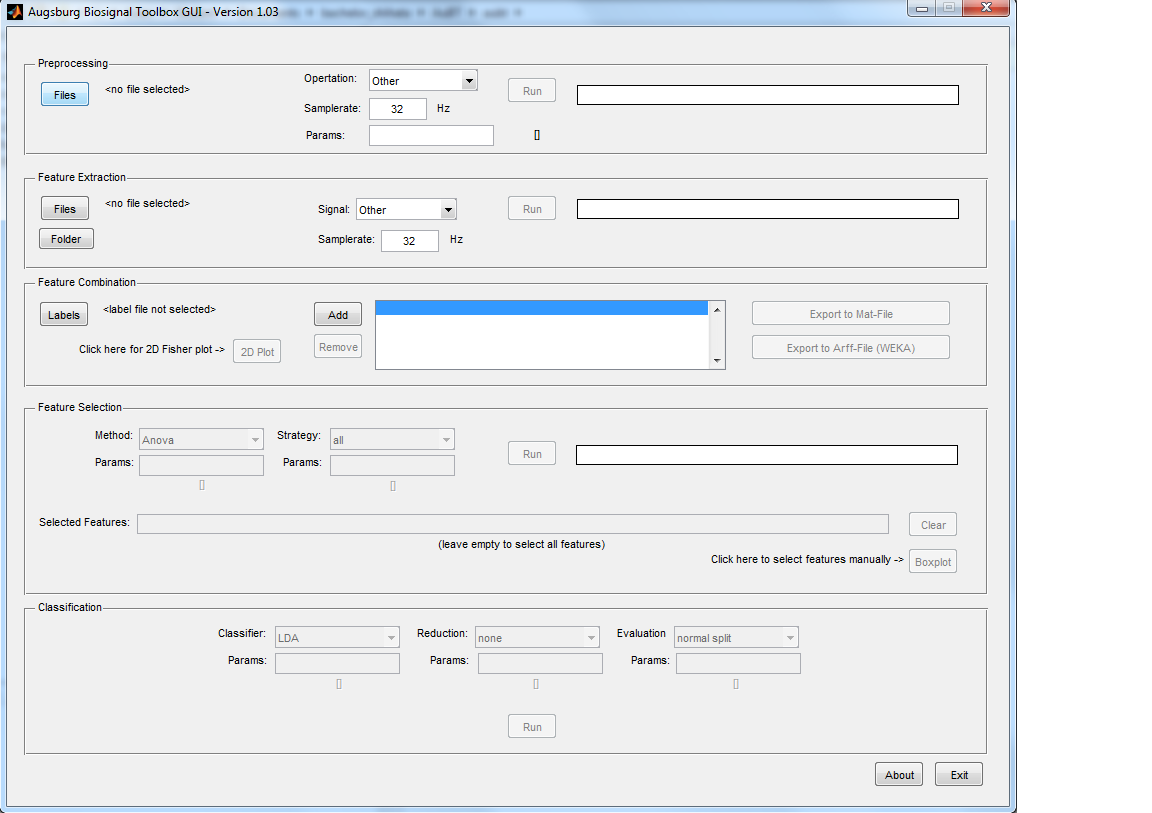
\includegraphics[width=0.6\textwidth]{aubt1.png}
	\caption{Final version of the AuBT toolbox}
	\label{fig:aubt1}
\end{figure}

First the preprocessing that accompanied the DEAP dataset was added, to be able to apply it to future signals.
\begin{figure}[h]
	\centering
	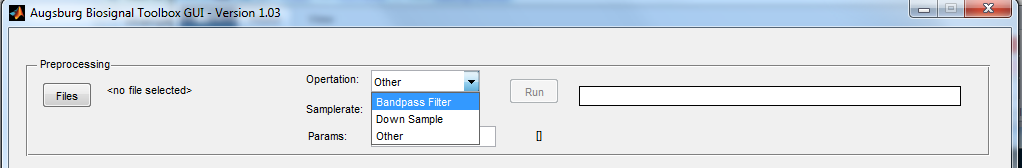
\includegraphics[width=0.6\textwidth]{aubt2.png}
	\caption{Preprocessing area of the GUI}
	\label{fig:aubt2}
\end{figure}
Feature extraction specific for EEG signals was implemented. The toolbox now recognizes specific EEG channels for spacial features, as well as a generic EEG channel if only temporal features are of interest.

\begin{figure}[h]
	\centering
	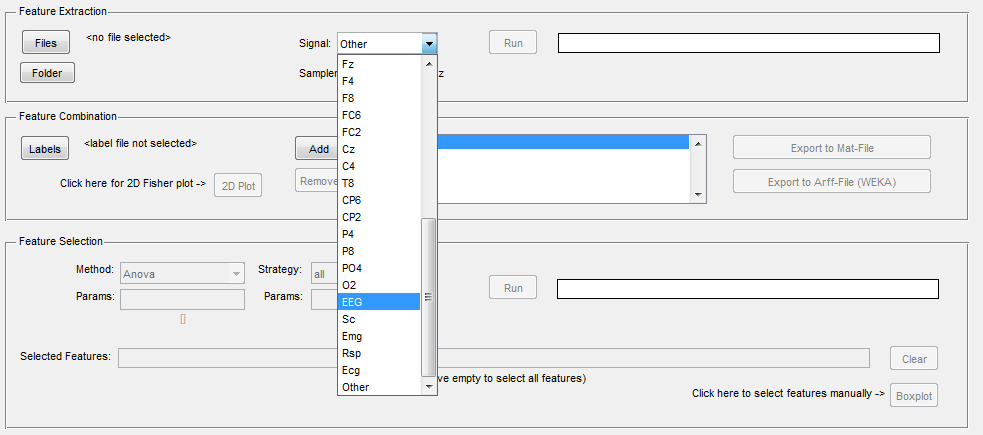
\includegraphics[width=0.6\textwidth]{aubt3.png}
	\caption{Feature selection with newly added support for EEG signals}
	\label{fig:aubt3.jpg}
\end{figure}

Finally the Gaussian classifier was included in the list of classifiers, with the other previously implemented classifiers.

\begin{figure}[h]
	\centering
	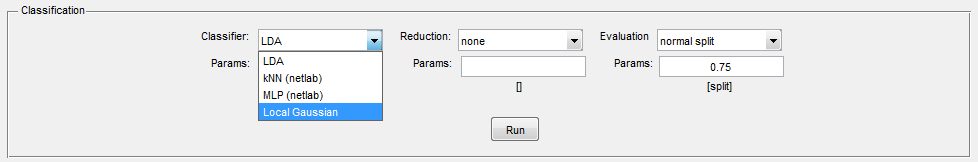
\includegraphics[width=0.8\textwidth]{aubt4.png}
	\caption{Newly added Gaussian classifier}
	\label{fig:aubt4.jpg}
\end{figure}


%******************************************************************************
% BACK MATTER
%******************************************************************************
\backmatter

%******************************************************************************
% LIST OF SYMBOLS
%******************************************************************************
%\normalfont
%\clearpage
%\chapter[List of Symbols and Abbreviations]{List of Symbols and Abbreviations}
%\begin{center}
%\small
%\begin{longtable}{lp{3.0in}c}
%\toprule
%\multicolumn{1}{c}{Abbreviation} & \multicolumn{1}{c}{Description}\\ \midrule\addlinespace[2pt] \endhead
%\bottomrule\endfoot
%XML & E\textbf{X}tensible \textbf{M}arkup \textbf{L}anguage \\
%XSD & \textbf{X}ML-\textbf{S}chema-\textbf{D}efinition \\
%SFXML & \textbf{S}cene\textbf{F}low E\textbf{X}tensible \textbf{M}arkup \textbf{L}anguage \\
%SFTXL & \textbf{S}cene\textbf{F}low \textbf{T}extual E\textbf{X}pression \textbf{L}anguage \\
%SCXML & \textbf{S}tate\textbf{C}hart E\textbf{X}tensible \textbf{M}arkup \textbf{L}anguage \\
%DOM & \textbf{D}ocument \textbf{O}bject \textbf{M}odel \\
%LR & \textbf{L}eft to \textbf{R}ightmost derivation \\
%LALR & \textbf{L}ook\textbf{A}head LR\\
%NPC & \textbf{N}on-\textbf{P}erson-\textbf{C}haracter\\
%ABL & \textbf{A} \textbf{B}ehavior \textbf{L}anguage\\
%\end{longtable}
%\end{center}

%******************************************************************************
% LIST OF FIGURES
%******************************************************************************
\normalfont
\clearpage
\listoffigures

%******************************************************************************
% LIST OF TABLES
%******************************************************************************
\normalfont
\clearpage
\listoftables

%******************************************************************************
% END DOCUMENT
%******************************************************************************
\end{document}
\end{document}
